\documentclass[tikz, border=3pt]{standalone}

\usepackage{amsmath,amssymb}
\usepackage{pgfplots}
\pgfplotsset{compat=1.18}
\usetikzlibrary{arrows.meta}
\usepackage{xcolor}

\definecolor{utnblue}{RGB}{0, 51, 102}
\definecolor{utnred}{RGB}{204, 0, 0}

\begin{document}
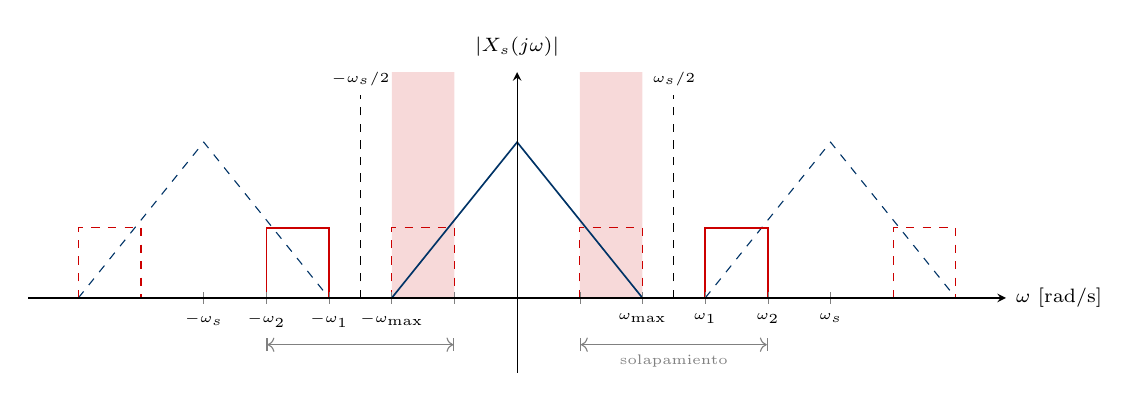
\begin{tikzpicture}[font=\scriptsize]

\begin{axis}[
    axis lines=middle,
    width=14cm, height=5.4cm,
    xmin=-3900, xmax=3900,
    ymin=-0.48, ymax=1.45,
    xtick={-2500,-2000,-1500,-1000,-500,500,1000,1500,2000,2500},
    xticklabels={$-\omega_s$,$-\omega_2$,$-\omega_1$,$-\omega_{\max}$,,,
                 $\omega_{\max}$,$\omega_1$,$\omega_2$,$\omega_s$},
    ytick=\empty,
    tick label style={font=\tiny},
    label style={font=\scriptsize},
    every axis x label/.style={at={(ticklabel* cs:1)}, anchor=west},
    every axis y label/.style={at={(ticklabel* cs:1.02)}, anchor=south},
    xlabel={$\omega$ [rad/s]},
    ylabel={$|X_s(j\omega)|$},
    enlargelimits=false,
    clip mode=individual,
    axis on top,
]

% ---- zonas de la banda util contaminadas por el ruido ----
\addplot[draw=none, fill=utnred!15]
    coordinates {(500,0) (1000,0) (1000,1.45) (500,1.45)} \closedcycle;
\addplot[draw=none, fill=utnred!15]
    coordinates {(-1000,0) (-500,0) (-500,1.45) (-1000,1.45)} \closedcycle;

% ---- banda util: copia central y replicas ----
\addplot[utnblue, semithick] coordinates {(-1000,0) (0,1) (1000,0)};
\addplot[utnblue, dashed, thin] coordinates {(1500,0) (2500,1) (3500,0)};
\addplot[utnblue, dashed, thin] coordinates {(-3500,0) (-2500,1) (-1500,0)};

% ---- ruido: bandas originales (rectangulares, como en el enunciado) ----
\addplot[utnred, semithick] coordinates {(1500,0) (1500,0.45) (2000,0.45) (2000,0)};
\addplot[utnred, semithick] coordinates {(-2000,0) (-2000,0.45) (-1500,0.45) (-1500,0)};

% ---- ruido: replicas que caen en la banda util ----
\addplot[utnred, dashed, thin] coordinates {(500,0) (500,0.45) (1000,0.45) (1000,0)};
\addplot[utnred, dashed, thin] coordinates {(-1000,0) (-1000,0.45) (-500,0.45) (-500,0)};

% ---- ruido: replicas lejanas ----
\addplot[utnred, dashed, thin] coordinates {(3000,0) (3000,0.45) (3500,0.45) (3500,0)};
\addplot[utnred, dashed, thin] coordinates {(-3500,0) (-3500,0.45) (-3000,0.45) (-3000,0)};

% ---- frecuencia de Nyquist ----
\addplot[black, dashed, thin] coordinates {(1250,0) (1250,1.3)};
\addplot[black, dashed, thin] coordinates {(-1250,0) (-1250,1.3)};
\node[font=\tiny, anchor=south] at (axis cs:1250,1.3) {$\omega_s/2$};
\node[font=\tiny, anchor=south] at (axis cs:-1250,1.3) {$-\omega_s/2$};

% ---- franja de solapamiento entre la copia central y la vecina ----
\draw[|<->|, gray, thin] (axis cs:500,-0.30) -- (axis cs:2000,-0.30)
    node[midway, below, font=\tiny, gray] {solapamiento};
\draw[|<->|, gray, thin] (axis cs:-2000,-0.30) -- (axis cs:-500,-0.30);

\end{axis}

\end{tikzpicture}
\end{document}
